\part[author={\protect\insertauthor},label={chap:overview}]{Overview of the Compilation Theory}

\begin{graphicspathcontext}{{./chapters/chapter1/imgs/raw/},{./chapters/chapter1/imgs/auto/}}
\begin{bibunit}[apalike]

\tableofcontentslide

\section{Introduction}

\begin{frame}{{Base Principles} of Computing}
	\begin{itemize}
	\item Programming languages are \emph{notations} for describing computations to people and to machines
	\item All the software running on all the computers was written in some \emph{programming language}
	\item Before a program can be run, it first must be \emph{translated} into a form in which it can be \emph{executed} by a computer
	\item The software systems that do this translation are called a \emph{compiler}
	\end{itemize}
\end{frame}

\begin{frame}{Goal of this Chapter}
	\alertbox{Overview of the principles, architecture and implementation of a simple compiler}
	\vspace{1cm}
	\centering With this chapter, you may understand the key points of language theory
\end{frame}

\section{Programming languages}
\subsectiontableofcontentslide

\subsection{Brief history}

\figureslide{{Brief History} of Main Programming Languages}{timeline}

\sidenote{Figure by \'Eric L\'ev\'enez --- \url{www.levenez.com/lang}}
\figureslide[scale=1]{{More than 8,900} Programming Languages}{brief_history_of_languages}

\subsection{Classifications and types of programming languages}
\subsectiontableofcontentslide

\begin{frame}{Generations of Programming Languages}
	\begin{columns}
		\begin{column}{.5\linewidth}
			\begin{rightanchorblock}{Machine languages}{1GL}
				0100101101
			\end{rightanchorblock}
			\vspace{0.5cm}
			\begin{rightanchorblock}{Assembly languages}{2GL}
				Intel, Motorola\dots
			\end{rightanchorblock}
			\vspace{0.5cm}
			\begin{rightanchorblock}{High-level languages}{3GL}
				Fortran, Cobol, Lisp, C, C++, C\#, Java\dots
			\end{rightanchorblock}
		\end{column}
		\begin{column}{.5\linewidth}
			\begin{leftanchorblock}{Domain-specific languages}{4GL}
				SQL, Postscript, HTML, SARL\dots
			\end{leftanchorblock}
			\vspace{0.5cm}
			\begin{leftanchorblock}{Logic and constraint languages}{5GL}
				Prolog, OPS5, Object-Z\dots
			\end{leftanchorblock}
		\end{column}
	\end{columns}
\end{frame}

\begin{frame}{Imperative vs. Declarative Language}
	\fancybox[width=.45\linewidth]{Imperative}{%
		\emph{HOW} a computation is to be done \\
		Notion of program state, statements and control flow \\
		(C, C++, C\#, Java)
	}{howto}{}
	\hfill
	\fancybox[width=.45\linewidth]{Declarative}{%
		\Emph{WHAT} computation is to be done \\
		Description of the logic of computation but not its control flow \\
		(ML, Haskell, Prolog, SQL, HTML)
	}{whatthis}{}
\end{frame}

\sidenote{\cite{Firmeprogramming.2013} - \url{www.vimustar.com}}
\animatedfigureslide{Types of Programming Languages}{programming-paradigms}

\figureslide{Static vs. Dynamic Typing}{static_dynamic}

\begin{frame}{Strongly vs. Weakly Typed Language}
	\alertbox*{A variable may be associated to a type of values, i.e. the definition of a set of values}
	\vspace{.5cm}
		\fancybox[vpos=b]{Strongly Typed}{%
			Single type for each variable \\
			Type defined at compile time
		}{strongly-typed}{}
		\raisebox{\height}{\larger\begin{tabular}{@{}l@{}p{2cm}@{}}
			\textcolor{CIADgreen}{$\oplus$} & reliable \\
			\textcolor{CIADmagenta}{$\ominus$} & tedious to write type annotations \\
		\end{tabular}}
		\hfill
		\fancybox[vpos=b]{Weakly Typed}{%
			Variable type depends on the run-time context \\
			Values are converted at run-time
		}{weakly-typed}{}
		\raisebox{\height}{\larger\begin{tabular}{@{}l@{}p{2cm}@{}}
			\textcolor{CIADgreen}{$\oplus$} & flexible \\
			\textcolor{CIADmagenta}{$\ominus$} & unexpected run-time errors \\
		\end{tabular}}
\end{frame}

\subsection{Basics of programming languages}

\subsubsection{Definitions}
\subsubsectiontableofcontentslide*

\sidecite{Sethi.1996, Scott.2006}
\begin{frame}[t]{Several Key Definitions}
	\begin{definitionblock}{Name}
		A string of characters that refers to a thing in the program
	\end{definitionblock}
	\begin{definitionblock}{Identifier}
		A string of characters that refers to an entity (data object, procedure, class, type) \begin{itemize}
			\item All identifiers are names; but not all names are identifiers
			\item \id{x.y} is a name but not an identifier, and \id{x} and \id{y} are identifiers.
		\end{itemize}
	\end{definitionblock}
	\begin{definitionblock}{Variable}
		A particular location of the store of the values at run-time. \\
		A variable is denoted by a name. Each declaration of an identifier introduces a new variable.
	\end{definitionblock}
	\begin{definitionblock}{Keyword}
		An identifier that has a particular meaning to the programming language
	\end{definitionblock}
\end{frame}

\sidecite{Sethi.1996, Scott.2006}
\begin{frame}{Several Key Definitions \insertcontinuationtext}
	\begin{definitionblock}{Program or Subprogram}
		A sequence of instructions and statements
	\end{definitionblock}
	\begin{definitionblock}{Procedure}
		A subprogram with a name and formal parameters that may be called
	\end{definitionblock}
	\begin{definitionblock}{Function}
		A procedure that may return a value of some type (the``return type'')
	\end{definitionblock}
	\begin{definitionblock}{Method}
		A procedure or a function inside a class in object-oriented languages
	\end{definitionblock}
	\begin{alertblock}{Caution}
	In the C-family languages, all the subprograms are functions; and a function is enabled to return nothing (\kw{void})
	\end{alertblock}
\end{frame}

\sidecite{Sethi.1996, Scott.2006}
\begin{frame}{Several Key Definitions \insertcontinuationtext}
	\begin{definitionblock}{Declaration}
		Tells us about the type of an element. \inlineexample{\code{\kw{int} i;}}
	\end{definitionblock}
	\begin{definitionblock}{Definition}
		Tells us about the value of an element. \inlineexample{\code{i = 1;}}
	\end{definitionblock}
	\begin{definitionblock}{Signature of a procedure/function}
		The declaration of the procedure/function \\
		Composed of: a return type, an identifier, and a collection of parameter declarations
	\end{definitionblock}
	\begin{example}\smaller In C++: \begin{itemize}
		\item a method is declared in a \code{.hpp} file
		\item a method is defined in a \code{.cpp} file
		\end{itemize}
	\end{example}
\end{frame}

\subsubsection{Environment and state}

\begin{frame}{Environment and State}
	Association of names with locations in memory (the store) and then with values is described by two mappings:
	\begin{description}
	\item[Environment] mapping from names to locations in the store.
	\item[State] mapping from locations in store to their values.
	\end{description}
	\vfill
	\begin{center}
	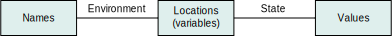
\includegraphics[width=.9\linewidth]{environment_state}
	\end{center}
\end{frame}

\begin{frame}[fragile]{Example of Environment and State}
	\begin{lstlisting}[language=C,basicstyle=\normalcolor\smaller\smaller]
	int i;         /* global i */
	...
	void f(...) {
	  int i;       /* local i */
	  ...
	  i = 3;       /* use of local i */
	  ...
	}
	...
	x = i + 1;     /* use of global i */
	\end{lstlisting}
	\vfill
	\begin{center}
	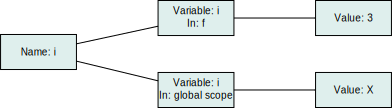
\includegraphics[width=.8\linewidth]{environment_state_example}
	\end{center}
\end{frame}

\subsubsection{Static or dynamic policy}
\begin{frame}{Static or Dynamic Policy}
	\alertbox{One of the most important issues when designing a compiler is related to the decisions the compiler make about the program}
	\vspace{1cm}
	\begin{definitionblock}{Static Policy}
	A program uses a policy that enables the compiler to decide an issue; \emph{the decision could be decided at compile time.}
	\end{definitionblock}
	\vspace{.5cm}
	\begin{definitionblock}{Dynamic Policy}
	The decision can be made when we execute the program; \emph{the decision is required at run time.}
	\end{definitionblock}
\end{frame}

\sidecite{Church.1941, Frege.1967, Wexelblat.1981}
\begin{frame}{Example: Declaration Scope}
	\begin{definitionblock}{Static Scope}
		A language uses a static scope if it is possible to determine the scope of a declaration by looking only at the program (C, Java\dots)
	\end{definitionblock}
	\vspace{1cm}
	\begin{definitionblock}{Dynamic Scope}
		With dynamic scope, as the program runs, the same use of a variable x could refer to any of several different declarations of x (Perl, PHP\dots)
	\end{definitionblock}
\end{frame}

\begin{frame}{{``static'' Term Use} in Java}
	\begin{center}
		\code{\kw{public} \kw{static} \kw{int} x = 1;}
	\end{center}
	\vfill
	\begin{itemize}
	\item Here \kw{static} refers not to the scope of the variable, but rather to the ability of the compiler to determine the location in memory
	\vfill
	\item If \kw{static} is omitted each object has this variable and the compiler cannot determine where it is in advance
	\end{itemize}
\end{frame}

\begin{frame}{{}{Are Environment and State Mappings Dynamic or Static?}}
	\alertbox*{Environment and state mappings are often dynamic}
	\vspace{.5cm}
	\begin{block}{Static or Dynamic Environment Mapping?}
	\begin{itemize}
	\item Most of binding names to locations are \emph{dynamic}
	\item Some declarations (\eg global \id{i}) are determine at compile time; they are static
	\end{itemize}
	\end{block}
	\vspace{.5cm}
	\begin{block}{Static or Dynamic State Mapping?}
	\begin{itemize}
	\item Most of binding locations to values are \emph{dynamic} because it is impossible to determine the location until we run the program
	\item Declared constants are an exception
	\end{itemize}
	\end{block}
\end{frame}

\subsubsection{Parameter-passing mechanisms}

\begin{frame}{{Parameter-passing} Mechanisms}
	\alertbox*{All programming languages have the notion of procedur; but they can differ in how these procedures get their arguments}
	\vspace{1cm}
	\alertbox{How are the actual parameters (the parameters used in the call of a procedure) associated with the formal parameters (those used in the procedure definition)?}
	\vspace{1cm}
	\begin{columns}
		\begin{column}{.33\linewidth}
			\simplebox{\textcircled{1} Call-by-value}
		\end{column}
		\begin{column}{.33\linewidth}
			\simplebox{\textcircled{2} Call-by-reference}
		\end{column}
		\begin{column}{.33\linewidth}
			\simplebox{\textcircled{3} Call-by-name}
		\end{column}
	\end{columns}
\end{frame}

\begin{frame}[t]{\textcircled{1} Call-by-value}
	\begin{block}{Principle}
		\begin{itemize}
		\item Actual parameter is evaluated or copied
		\item Value is in the location of the formal parameter
		\end{itemize}
	\end{block}
	\begin{block}{Constraints}
		\begin{itemize}
			\item Changes to formal parameter is local to the procedure
			\item Actual parameters themselves cannot be changed
		\end{itemize}
	\end{block}
	\begin{example}
		Used in C and Java; and the default option in C++
	\end{example}
	\begin{alertblock}{Caution}
		In Java, all the object variables are references (or pointers) to the objects. Parameters are passed with the call-by-value policy, not the call-by-reference
	\end{alertblock}
\end{frame}

\begin{frame}{\textcircled{2} Call-by-reference}
	\begin{block}{Principle}
		\begin{itemize}
			\item Address of the actual parameter is passed to the callee as the value of the corresponding formal parameter
			\item Uses of the formal parameter are implemented by following the pointer to the location indicated by the caller
		\end{itemize}
	\end{block}
	\begin{block}{Constraints}
		\begin{itemize}
			\item Changes to the formal parameter thus appear as changes to the actual parameter
		\end{itemize}
	\end{block}
\end{frame}

\begin{frame}{\textcircled{3} Call-by-name}
	\begin{block}{Principle}
		\begin{itemize}
			\item It requires that the callee execute as if the actual parameter were substituted literally for the formal parameter in the code of the callee
			\item Uses of the formal parameter are implemented by following the pointer to the location indicated by the caller
		\end{itemize}
	\end{block}
	\vspace{1cm}
	\begin{example}
		Macro-functions in the C-family languages use this parameter passing mechanism
	\end{example}
\end{frame}


\section[Language processor]{What is a language processor?}

\sectiontableofcontentslide

\begin{frame}{{What is a} Compiler?}
	\begin{itemize}
	\item Read a program in one language --- the source language
	\item Translate it into an equivalent program in a \Emph{low-level language} --- the target language
	\vfill
	\item Report any errors in the source program that are detected during the translation process
	\end{itemize}
	\vfill
	\begin{center}
		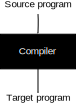
\includegraphics[width=.2\linewidth]{compiler_processor}
	\end{center}
\end{frame}

\begin{frame}{{What is a} Transpiler?}
	\begin{itemize}
		\item Read a program in one language --- the source language
		\item Translate it into an equivalent program in \Emph{another language that is not low-level} --- the target language
		\vfill
		\item Report any errors in the source program that are detected during the translation process
	\end{itemize}
	\vfill
	\begin{center}
		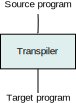
\includegraphics[width=.2\linewidth]{transpiler_processor}
	\end{center}
\end{frame}

\begin{frame}{Running the program}
	If the target program is an executable machine-language program, it can then be called by the user to process inputs and produce outputs
	\vfill
	\begin{center}
		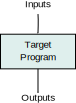
\includegraphics[width=.2\linewidth]{run_program}
	\end{center}
\end{frame}

\begin{frame}{{What is an} Interpreter?}
	\begin{itemize}
	\item A kind of language processor
	\item Does not produce a target program
	\item Directly execute the operations specified in the source program on inputs supplied by the user
	\end{itemize}
	\vfill
	\begin{center}
		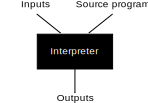
\includegraphics[width=.4\linewidth]{interpreter_processor}
	\end{center}
\end{frame}

\begin{frame}{{What is an} Hybrid Compiler?}
	\begin{itemize}
	\item Combine compilation and interpretation
	\item Generate intermediate program in a platform-independent language
	\item Execute the intermediate program in a platform-dependent virtual machine
	\end{itemize}
	\vfill
	\begin{center}
		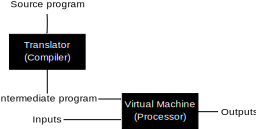
\includegraphics[width=.7\linewidth]{hybrid_processor}
	\end{center}
\end{frame}

\begin{frame}{Properties of the Language Processors}
	\begin{smaller}
	\begin{block}{Compiler \vs Transpiler \vs Interpreter}
	\begin{itemize}
	\item Compiler and transpiler is faster than interpreter at mapping inputs to outputs
	\item Interpreter gives better error diagnostics than compiler, because it execute the source program statement by statement (no code optimization)
	\end{itemize}
	\end{block}
	\vspace{1cm}
	\begin{block}{Hybrid Compiler}
	\begin{itemize}
	\item Compile on \emph{one machine}, execute the generated program on \emph{another machine}
	\item To be faster, use just-in-time compilers to translate intermediate programs into machine language and avoid the interpretation, \eg the Oracle's Java Runtime Environment
	\end{itemize}
	\end{block}
	\end{smaller}
\end{frame}

\begin{frame}<1>[t]{Toolchain}
	\begin{itemize}
	\item Several other programs may be required to create an executable target program
	\item They compose the toolchain of the compiler
	\end{itemize}
	\putat(40,-150){\includeanimatedfigure[width=.8\linewidth]{toolchain}}
\end{frame}

\begin{frame}<2>[t]{Preprocessor in the Toolchain}
	\begin{smaller}
	\begin{block}{\smaller Goals}
	\begin{itemize}
	\item To collect the different files of the program's modules to compile
	\item To expand shorthands, macros into statements
	\end{itemize}
	\end{block}
	\end{smaller}
	\putat(40,-150){\includeanimatedfigure[width=.8\linewidth]{toolchain}}
\end{frame}

\begin{frame}<3>[t]{Compiler in the Toolchain}
	\begin{smaller}
	\begin{block}{\smaller Goals}
	\begin{itemize}
	\item To produce an assembly-language program from the modified source program
	\item Assembly-language is easier to produce and debug
	\end{itemize}
	\end{block}
	\end{smaller}
	\putat(40,-150){\includeanimatedfigure[width=.8\linewidth]{toolchain}}
\end{frame}

\begin{frame}<4>[t]{Assembler in the Toolchain}
	\begin{smaller}
	\begin{block}{\smaller Goals}
	\begin{itemize}
	\item To translate to a machine code that could be relocated in the code segment of the program
	\item Code segment: the part of the memory where machine code is store
	\end{itemize}
	\end{block}
	\end{smaller}
	\putat(40,-150){\includeanimatedfigure[width=.8\linewidth]{toolchain}}
\end{frame}

\begin{frame}<5>[t]{Linker in the Toolchain}
	\begin{smaller}
	\begin{block}{\smaller Goals}
	\begin{itemize}
	\item To resolve external memory addresses, where the code in one file (library or object) may refer to a location in another file (library or object)
	\end{itemize}
	\end{block}
	\end{smaller}
	\putat(40,-150){\includeanimatedfigure[width=.8\linewidth]{toolchain}}
\end{frame}

\section{Process of a compiler}

\sectiontableofcontentslide

\begin{frame}<9>{Process of a Compiler}
	\putat*(340,-197){\includeanimatedfigure[width=2.5cm]{compiler_structure}}
	\begin{minipage}{.8\linewidth}
	\begin{block}{Analysis}
	\begin{itemize}
	\item The \emph{analysis} breaks up the source program into constituent pieces and imposes a grammatical structure to them.
	\item It detects if the source program is ill formed or semantically unsound.
	\item It collects informations about the source program and stores it in a data structure called symbol table.
	\item This part is often called the \emph{front end of the compiler}.
	\end{itemize}
	\end{block}
	\end{minipage}
\end{frame}

\begin{frame}<10>{Process of a Compiler}
	\putat*(340,-197){\includeanimatedfigure[width=2.5cm]{compiler_structure}}
	\begin{minipage}{.8\linewidth}
	\begin{block}{Synthesis}
	\begin{itemize}
	\item The \emph{synthesis} constructs the desired target program from the intermediate representation and the information in the symbol table.
	\item This part is often called the \emph{back end of the compiler}.
	\end{itemize}
	\end{block}
	\end{minipage}
\end{frame}

\begin{frame}<2>{{Lexical Analysis} or Scanning}
	\putat*(340,-197){\includeanimatedfigure[width=2.5cm]{compiler_structure}}
	\begin{minipage}{.8\linewidth}
	\begin{itemize}
	\item Reads the stream of characters making up the source program
	\item Groups the characters into meaningful sequences called \emph{lexemes}
	\item Output for each lexeme:
		\begin{center}
			\code{token={\textless}token-name, attribute-value{\textgreater}}
		\end{center}
		\begin{itemize}
		\item \code{token-name}: the identifier of the token
		\item \code{attribute-value}: entry in the symbol table for this token
		\end{itemize}
		\end{itemize}
	\end{minipage}
\end{frame}

\begin{frame}<2>{Example of Scanning}
	\putat*(340,-197){\includeanimatedfigure[width=2.5cm]{compiler_structure}}
	\begin{small}
	\begin{minipage}{.8\linewidth}
	\begin{center}
		\code{position = initial + rate * 60}
	\end{center}
	\begin{tabularx}{\linewidth}{|l|X|}
		\hline
		\tabularheading\chead{Lexeme}&\chead{Token} \\
		\hline
		\code{position} & \code{{\textless}id,1{\textgreater}} 
			\begin{itemize}
				\item \code{id}: abstract symbol standing for ``identifier''
				\item \code{``1''}: points to the symbol-table entry for position
			\end{itemize} \\
		\hline
		\code{=} & \code{{\textless}={\textgreater}} \\
		\hline
		\code{initial} & \code{{\textless}id,2{\textgreater}} \\
		\hline
		\code{+} & \code{{\textless}+{\textgreater}} \\
		\hline
		\code{rate} & \code{{\textless}id,3{\textgreater}} \\
		\hline
		\code{*} & \code{{\textless}*{\textgreater}} \\
		\hline
		\code{60} & \code{{\textless}number,60{\textgreater}} \\
		\hline
	\end{tabularx}
	\end{minipage}
	\end{small}
\end{frame}

\begin{frame}<2>{Example of Scanning}
	\putat*(340,-197){\includeanimatedfigure[width=2.5cm]{compiler_structure}}
	\putat(0,-120){\includeanimatedfigure[width=.65\linewidth]{compiler_cycle_example}}
\end{frame}

\begin{frame}{Symbol Table}
	\begin{definitionblock}{Symbol Table}
		Central data structure containing a record for each variable name, with record fields for the attributes associated to the name
	\end{definitionblock}
	\vspace{.5cm}
	\begin{definitionblock}{Record Attribute}
		Information about the storage allocated for a name: type, scope, number and types of the formal parameters, the method of passing each argument, and the type of the returned value
	\end{definitionblock}
	\vspace{.5cm}
	\begin{alertblock}{Caution}
		Should be designed to allow the compiler to find the record for each name quickly and to store or retrieve data from that record quickly
	\end{alertblock}
\end{frame}

\begin{frame}{Symbol Table and Scope}
	\alertbox*{Scopes are implemented by setting up a separate symbol table for each scope}
	\vspace{.25cm}
	\begin{block}{Principle}
		The \emph{most-closely nested rule for blocks} permits to define a data structure, which is based on \emph{chained symbol tables}.
	\end{block}
	\begin{center}
		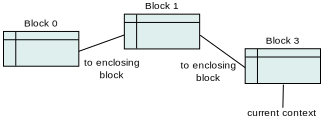
\includegraphics[width=.8\linewidth]{symbol_table_chain}
	\end{center}
\end{frame}

\begin{frame}[t,fragile]{{Simple Java Implementation} of the Symbol Table Chain}
	\begin{lstlisting}[language=java,basicstyle=\normalcolor\smaller\smaller]
/** Define the properties of a single symbol. */
public class Symbol {
 public final String lexeme;
 public Type type;
 public Address storagePosition;
 public Symbol(String lexeme) { this.lexeme = lexeme; }
}

/** Define a symbol table. */
public class SymbolTable {

 /** Collection of the symbol in the current context. */
 private final Map<String,Symbol> table = new TreeMap<String,Symbol>();

 /** Reference to the symbol table that is associated to the enclosing scope. */
 private final SymbolTable enclosingEnvironment;

 /** Constructor. */
 private SymbolTable(SymbolTable enclosingEnvironment) {
     this.enclosingEnvironment = enclosingEnvironment;
 }
 //....
	\end{lstlisting}
\end{frame}

\begin{frame}[t,fragile]{{Simple Java Implementation} of the Symbol Table Chain}
	\begin{lstlisting}[language=java,basicstyle=\normalcolor\smaller\smaller]
 /** Declare a symbol in the current context. */
 public void declare(String identifier, Symbol symbol) {
     this.table.put(identifier, symbol);
 }

 /** Get the definition of a symbol in the current context,
     or in an enclosing scope. */
 public Symbol get(String identifier) {
     SymbolTable e = this;
     Symbol symbol;
     while (e!=null) {
         symbol = e.table.get(identifier);
         if (symbol != null) {
             return symbol;
         }
         e = e.enclosingEnvironment;
     }
     return null;
 }
 //....
	\end{lstlisting}
\end{frame}

\begin{frame}[t,fragile]{{Simple Java Implementation} of the Symbol Table Chain}
	\begin{lstlisting}[language=java,basicstyle=\normalcolor\smaller\smaller]
 /** Reference to the current symbol table.
     The reference is initialized with the
     root context (or the global context). */
 private static SymbolTable current = new SymbolTable(null);

 /** Replies the symbol table of the current context. */
 public static SymbolTable getCurrent() {
     return current;
 }

 /** Open a new context and create the corresponding
     symbol table. */
 public static void openContext() {
     current = new SymbolTable(current);
 }
 /** Close the current context. */
 public static void closeContext() {
     if (current.enclosingEnvironment!=null) {
         current = current.enclosingEnvironment;
     }
 }
}
	\end{lstlisting}
\end{frame}

\begin{frame}<3>{Syntax Analysis}
	\putat*(340,-197){\includeanimatedfigure[width=2.5cm]{compiler_structure}}
	\begin{minipage}{.8\linewidth}
		\alertbox*{Uses the tokens produced by the lexical analyzer to create an intermediate representation}
		\vspace{.5cm}
		\begin{block}{Syntax Tree}
			A typical representation is a syntax tree: \begin{description}
			\item[node] operation in the program
			\item[children] parameters of the operation
			\end{description}
			\vspace{1em}
			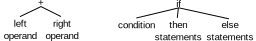
\includegraphics[width=\linewidth]{syntax_tree_example}
		\end{block}
	\end{minipage}
\end{frame}

\begin{frame}<3>{Example of Syntax Analysis}
	\putat*(340,-197){\includeanimatedfigure[width=2.5cm]{compiler_structure}}
	\putat(0,-120){\includeanimatedfigure[width=.65\linewidth]{compiler_cycle_example}}
\end{frame}

\begin{frame}<4>{Semantic Analysis}
	\putat*(340,-197){\includeanimatedfigure[width=2.5cm]{compiler_structure}}
	\begin{minipage}{.8\linewidth}
		\alertbox*{Uses the syntax tree and the information in the symbol table to check the source program for semantic consistency with the language definition}
		\vspace{.25cm}
		\begin{block}{Actions}
			\begin{itemize}
			\item Gathers type information and saves it in either the syntax tree and the symbol table
			\item Applies \emph{coercions}, or type conversions
			\end{itemize}
		\end{block}
		\vspace{.25cm}
		\begin{alertblock}{Type Checking}
			Important part of the semantic analyzer: the compiler checks that each operator has matching operands
		\end{alertblock}
	\end{minipage}
\end{frame}

\begin{frame}<4>{Example of Semantic Analysis}
	\putat*(340,-197){\includeanimatedfigure[width=2.5cm]{compiler_structure}}
	\putat(0,-120){\includeanimatedfigure[width=.65\linewidth]{compiler_cycle_example}}
\end{frame}

\begin{frame}<5>{{Intermediate Code} Generator}
	\putat*(340,-197){\includeanimatedfigure[width=2.5cm]{compiler_structure}}
	\begin{minipage}{.8\linewidth}
		\alertbox*{Many compilers generate an \emph{explicit low-level or machine-like intermediate representation}, which is a program for an abstract machine}
		\vspace{1cm}
		\begin{block}{Intermediate code}
			Two representations are generally used: \begin{itemize}
				\item Syntax tree
				\item Three-address code
			\end{itemize}
			that is easy to produce, and translate into the target machine
		\end{block}
	\end{minipage}
\end{frame}

\begin{frame}{{What is} Three-address Code?}
	\alertbox*{A sequence of assembly-like instructions with, at most, three operands per instruction. \\
		\code{{\textless}variable{\textgreater} = {\textless}operand1{\textgreater} {\textless}operator{\textgreater} {\textless}operand2{\textgreater}}}
	\begin{itemize}
	\item Each operand can act like a register
	\item The affectation operator is implicit and always present
	\end{itemize}
	\begin{alertblock}{Constraints}
		\begin{enumerate}
			\item At most one operator on the right side
			\item Temporary names are generated to hold the value computed by the three-address instruction
			\item Some instructions have fewer then three operands
		\end{enumerate}
	\end{alertblock}
\end{frame}

\begin{frame}<5>{Example of Intermediate Code Generation}
	\putat*(340,-197){\includeanimatedfigure[width=2.5cm]{compiler_structure}}
	\putat(0,-120){\includeanimatedfigure[width=.65\linewidth]{compiler_cycle_example}}
\end{frame}

\begin{frame}<6>{{Machine-Independent Code} Optimizer}
	\putat*(340,-197){\includeanimatedfigure[width=2.5cm]{compiler_structure}}
	\begin{minipage}{.8\linewidth}
		\alertbox*{Improves the intermediate code for better target code \\
			(faster, shorter, less power consumer\dots)}
		\vspace{.5cm}
		\begin{itemize}
		\item All the compilers include a machine-independent code optimizer
		\item Those that spent a large amount of time on this phase are named ``optimizing compilers''
		\end{itemize}
		\vspace{.5cm}
		\begin{block}{Note}
			Many of the simple optimizations permit to significantly improve the running time of the target program without too much time spent on this phase
		\end{block}
	\end{minipage}
\end{frame}

\figureslide{Example of Optimization}{intermediate_code_optim}

\begin{frame}<6>{Example of Machine-Independent Code Optimization}
	\putat*(340,-197){\includeanimatedfigure[width=2.5cm]{compiler_structure}}
	\putat(0,-120){\includeanimatedfigure[width=.65\linewidth]{compiler_cycle_example}}
\end{frame}

\begin{frame}<7>{Code Generator}
	\putat*(340,-197){\includeanimatedfigure[width=2.5cm]{compiler_structure}}
	\begin{minipage}{.8\linewidth}
		\alertbox*{Maps an intermediate representation into the target language}
		\vspace{.5cm}
		\begin{itemize}
		\item If the target language is machine code, registers or memory locations are selected for each variables used by the program
		\item Then, the intermediate instructions are translated into sequences of machine instructions that perform the same tasks
		\vspace{.5cm}
		\item A crucial aspect is the judicious assignment of registers to hold variables
		\end{itemize}
	\end{minipage}
\end{frame}

\begin{frame}{Example of Code Generation}
	\begin{itemize}
	\item Assumes that R1 and R2 are registers
	\item Variables are mapped to registers so that they can be easily used for the generation of the next instructions
	\end{itemize}
	\vspace{.25cm}
	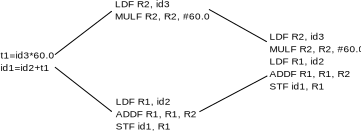
\includegraphics[width=\linewidth]{code_generator_example}
\end{frame}

\begin{frame}<7>{Example of Code Generation}
	\putat*(340,-197){\includeanimatedfigure[width=2.5cm]{compiler_structure}}
	\putat(0,-120){\includeanimatedfigure[width=.65\linewidth]{compiler_cycle_example}}
\end{frame}

\section{Tools to create a compiler}
\sectiontableofcontentslide

\begin{frame}{Tools to Create a Compiler}
	\alertbox*{Several tools are available to help the compiler writer to build his compiler}
	\vspace{.5cm}
	\fancybox{Scanner generators}{Lexical analyzers from a reg-ex description tokens \\
	(Flex, JFlex\dots)}{scanner-icon}{1}
	\hfill
	\fancybox{Parser generators}{Syntax analyzers from grammar \\
	(Yacc, JavaCC, Bison\dots)}{parser-icon}{2}
	\hfill
	\fancybox{Syntax-directed translation engines}{Parse-tree walkthrough routines for intermediate code generation}{assembly-icon}{3}
\end{frame}

\begin{frame}{Tools to Create a Compiler \insertcontinuationtext}
	\fancybox{Code-generator generators}{Procedures for generating target machine code from intermediate code}{machine-code-icon}{4}
	\hfill
	\fancybox{Data-flow analysis engines}{Help for management of value exchange between compiler components}{data-flow-icon}{5}
	\hfill
	\fancybox{Construction toolkits}{Include the other tools and IDE integration (Xtext\dots)}{toolkit-icon}{6}
\end{frame}

\section{Conclusion}
\sectiontableofcontentslide

\begin{frame}[t]{{Key Concepts} in the Chapter}
	\begin{description}
	\item[Language Processors] An integrated software development environment: compilers, interpreters, linkers, loaders, debuggers, profilers.
	\item[Compiler Phases] Sequence of phases, each of which transforms the source program from one intermediate representation to another.
	\item[Machine and Assembly Languages] Machine languages were the first-generation programming languages, followed by assembly languages.
	\item[Code Optimization] the science of improving the efficiency of code in both complex and very important. It is a major portion of the study of compilation.
	\item[Higher-Level Languages] Programming languages take on progressively more of the tasks that formerly were left to the programmer: memory management, type-consistency\dots
	\item[Environments] The association of names with locations in memory and then with values can be described in terms of environments.
	\item[Parameter Passing] Parameters are passed from a calling procedure to the callee either by value or by reference.
	\end{description}
\end{frame}

\begin{frame}[t]{{Key Concepts} in the Chapter \insertcontinuationtext}
	\begin{description}
		\item[Aliasing] When parameters are (effectively) passed by reference, two formal parameters can refer to the same object.
		\item[Compiler Front End] The part of the compiler that is dedicated to the analysis phases. The compiler front end takes the source program, breaks it to token, analyzes the grammar, detects errors and inconsistencies, and generate an intermediate representation.
		\item[Compiler Back End] The part of the compiler that is dedicated to the synthesis phases. The compiler back end takes the intermediate representation, generates assembly and machine code.
		\item[Lexical Analyzer] The lexical analyzer reads the input one character at a time and produces as output a stream of tokens. A token consists of a terminal symbol and attribute values.
		\item[Parsing] Parsing is the problem of figuring out how a string of terminals can be derived from the start symbol of the grammar by repeatedly replacing a nonterminal by the body of one of its productions.
	\end{description}
\end{frame}


\begin{frame}[t]{{Key Concepts} in the Chapter \insertcontinuationtext}
	\begin{description}
		\item[Parse Tree] A graphical tree representation of the productions that are matching a sequence of input tokens.
		\item[Intermediate Code] The result of the syntax analysis is a representation of the source program, called intermediate code. Two primary forms of intermediate code are illustrated: abstract syntax tree (similar to parse tree), and three-address code.
		\item[Symbol Table] A data structure that holds information about identifiers.
	\end{description}
\end{frame}

%%allowframebreaks
\begin{frame}[t]{{\bibname}\ of the Chapter}%
	\tiny%
	\putbib[chapters/chapter1/biblio]%
\end{frame}%

\end{bibunit}
\end{graphicspathcontext}